\documentclass[1p]{elsarticle_modified}
%\bibliographystyle{elsarticle-num}

%\usepackage[colorlinks]{hyperref}
%\usepackage{abbrmath_seonhwa} %\Abb, \Ascr, \Acal ,\Abf, \Afrak
\usepackage{amsfonts}
\usepackage{amssymb}
\usepackage{amsmath}
\usepackage{amsthm}
\usepackage{scalefnt}
\usepackage{amsbsy}
\usepackage{kotex}
\usepackage{caption}
\usepackage{subfig}
\usepackage{color}
\usepackage{graphicx}
\usepackage{xcolor} %% white, black, red, green, blue, cyan, magenta, yellow
\usepackage{float}
\usepackage{setspace}
\usepackage{hyperref}

\usepackage{tikz}
\usetikzlibrary{arrows}

\usepackage{multirow}
\usepackage{array} % fixed length table
\usepackage{hhline}

%%%%%%%%%%%%%%%%%%%%%
\makeatletter
\renewcommand*\env@matrix[1][\arraystretch]{%
	\edef\arraystretch{#1}%
	\hskip -\arraycolsep
	\let\@ifnextchar\new@ifnextchar
	\array{*\c@MaxMatrixCols c}}
\makeatother %https://tex.stackexchange.com/questions/14071/how-can-i-increase-the-line-spacing-in-a-matrix
%%%%%%%%%%%%%%%

\usepackage[normalem]{ulem}

\newcommand{\msout}[1]{\ifmmode\text{\sout{\ensuremath{#1}}}\else\sout{#1}\fi}
%SOURCE: \msout is \stkout macro in https://tex.stackexchange.com/questions/20609/strikeout-in-math-mode

\newcommand{\cancel}[1]{
	\ifmmode
	{\color{red}\msout{#1}}
	\else
	{\color{red}\sout{#1}}
	\fi
}

\newcommand{\add}[1]{
	{\color{blue}\uwave{#1}}
}

\newcommand{\replace}[2]{
	\ifmmode
	{\color{red}\msout{#1}}{\color{blue}\uwave{#2}}
	\else
	{\color{red}\sout{#1}}{\color{blue}\uwave{#2}}
	\fi
}

\newcommand{\Sol}{\mathcal{S}} %segment
\newcommand{\D}{D} %diagram
\newcommand{\A}{\mathcal{A}} %arc


%%%%%%%%%%%%%%%%%%%%%%%%%%%%%5 test

\def\sl{\operatorname{\textup{SL}}(2,\Cbb)}
\def\psl{\operatorname{\textup{PSL}}(2,\Cbb)}
\def\quan{\mkern 1mu \triangleright \mkern 1mu}

\theoremstyle{definition}
\newtheorem{thm}{Theorem}[section]
\newtheorem{prop}[thm]{Proposition}
\newtheorem{lem}[thm]{Lemma}
\newtheorem{ques}[thm]{Question}
\newtheorem{cor}[thm]{Corollary}
\newtheorem{defn}[thm]{Definition}
\newtheorem{exam}[thm]{Example}
\newtheorem{rmk}[thm]{Remark}
\newtheorem{alg}[thm]{Algorithm}

\newcommand{\I}{\sqrt{-1}}
\begin{document}

%\begin{frontmatter}
%
%\title{Boundary parabolic representations of knots up to 8 crossings}
%
%%% Group authors per affiliation:
%\author{Yunhi Cho} 
%\address{Department of Mathematics, University of Seoul, Seoul, Korea}
%\ead{yhcho@uos.ac.kr}
%
%
%\author{Seonhwa Kim} %\fnref{s_kim}}
%\address{Center for Geometry and Physics, Institute for Basic Science, Pohang, 37673, Korea}
%\ead{ryeona17@ibs.re.kr}
%
%\author{Hyuk Kim}
%\address{Department of Mathematical Sciences, Seoul National University, Seoul 08826, Korea}
%\ead{hyukkim@snu.ac.kr}
%
%\author{Seokbeom Yoon}
%\address{Department of Mathematical Sciences, Seoul National University, Seoul, 08826,  Korea}
%\ead{sbyoon15@snu.ac.kr}
%
%\begin{abstract}
%We find all boundary parabolic representation of knots up to 8 crossings.
%
%\end{abstract}
%\begin{keyword}
%    \MSC[2010] 57M25 
%\end{keyword}
%
%\end{frontmatter}

%\linenumbers
%\tableofcontents
%
\newcommand\colored[1]{\textcolor{white}{\rule[-0.35ex]{0.8em}{1.4ex}}\kern-0.8em\color{red} #1}%
%\newcommand\colored[1]{\textcolor{white}{ #1}\kern-2.17ex	\textcolor{white}{ #1}\kern-1.81ex	\textcolor{white}{ #1}\kern-2.15ex\color{red}#1	}

{\Large $\underline{12a_{0583}~(K12a_{0583})}$}

\setlength{\tabcolsep}{10pt}
\renewcommand{\arraystretch}{1.6}
\vspace{1cm}\begin{tabular}{m{100pt}>{\centering\arraybackslash}m{274pt}}
\multirow{5}{120pt}{
	\centering
	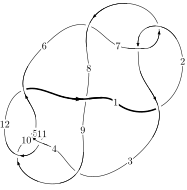
\includegraphics[width=112pt]{../../../GIT/diagram.site/Diagrams/png/1384_12a_0583.png}\\
\ \ \ A knot diagram\footnotemark}&
\allowdisplaybreaks
\textbf{Linearized knot diagam} \\
\cline{2-2}
 &
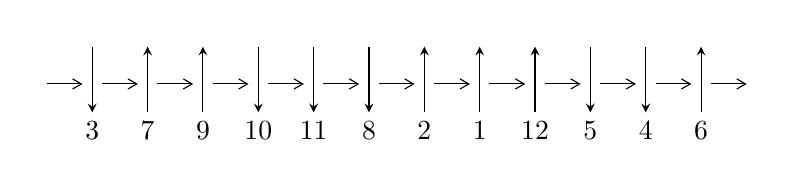
\begin{tikzpicture}[x=20pt, y=17pt]
	% nodes
	\node (C0) at (0, 0) {};
	\node (C1) at (1, 0) {};
	\node (C1U) at (1, +1) {};
	\node (C1D) at (1, -1) {3};

	\node (C2) at (2, 0) {};
	\node (C2U) at (2, +1) {};
	\node (C2D) at (2, -1) {7};

	\node (C3) at (3, 0) {};
	\node (C3U) at (3, +1) {};
	\node (C3D) at (3, -1) {9};

	\node (C4) at (4, 0) {};
	\node (C4U) at (4, +1) {};
	\node (C4D) at (4, -1) {10};

	\node (C5) at (5, 0) {};
	\node (C5U) at (5, +1) {};
	\node (C5D) at (5, -1) {11};

	\node (C6) at (6, 0) {};
	\node (C6U) at (6, +1) {};
	\node (C6D) at (6, -1) {8};

	\node (C7) at (7, 0) {};
	\node (C7U) at (7, +1) {};
	\node (C7D) at (7, -1) {2};

	\node (C8) at (8, 0) {};
	\node (C8U) at (8, +1) {};
	\node (C8D) at (8, -1) {1};

	\node (C9) at (9, 0) {};
	\node (C9U) at (9, +1) {};
	\node (C9D) at (9, -1) {12};

	\node (C10) at (10, 0) {};
	\node (C10U) at (10, +1) {};
	\node (C10D) at (10, -1) {5};

	\node (C11) at (11, 0) {};
	\node (C11U) at (11, +1) {};
	\node (C11D) at (11, -1) {4};

	\node (C12) at (12, 0) {};
	\node (C12U) at (12, +1) {};
	\node (C12D) at (12, -1) {6};
	\node (C13) at (13, 0) {};

	% arrows
	\draw[->,>={angle 60}]
	(C0) edge (C1) (C1) edge (C2) (C2) edge (C3) (C3) edge (C4) (C4) edge (C5) (C5) edge (C6) (C6) edge (C7) (C7) edge (C8) (C8) edge (C9) (C9) edge (C10) (C10) edge (C11) (C11) edge (C12) (C12) edge (C13) ;	\draw[->,>=stealth]
	(C1U) edge (C1D) (C2D) edge (C2U) (C3D) edge (C3U) (C4U) edge (C4D) (C5U) edge (C5D) (C6U) edge (C6D) (C7D) edge (C7U) (C8D) edge (C8U) (C9D) edge (C9U) (C10U) edge (C10D) (C11U) edge (C11D) (C12D) edge (C12U) ;
	\end{tikzpicture} \\
\hhline{~~} \\& 
\textbf{Solving Sequence} \\ \cline{2-2} 
 &
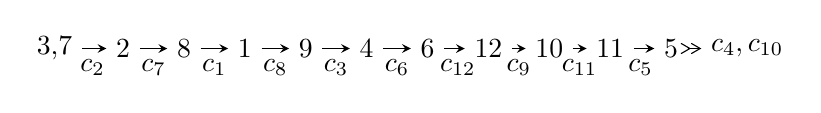
\begin{tikzpicture}[x=22pt, y=7pt]
	% node
	\node (A0) at (-1/8, 0) {3,7};
	\node (A1) at (1, 0) {2};
	\node (A2) at (2, 0) {8};
	\node (A3) at (3, 0) {1};
	\node (A4) at (4, 0) {9};
	\node (A5) at (5, 0) {4};
	\node (A6) at (6, 0) {6};
	\node (A7) at (7, 0) {12};
	\node (A8) at (8, 0) {10};
	\node (A9) at (9, 0) {11};
	\node (A10) at (10, 0) {5};
	\node (C1) at (1/2, -1) {$c_{2}$};
	\node (C2) at (3/2, -1) {$c_{7}$};
	\node (C3) at (5/2, -1) {$c_{1}$};
	\node (C4) at (7/2, -1) {$c_{8}$};
	\node (C5) at (9/2, -1) {$c_{3}$};
	\node (C6) at (11/2, -1) {$c_{6}$};
	\node (C7) at (13/2, -1) {$c_{12}$};
	\node (C8) at (15/2, -1) {$c_{9}$};
	\node (C9) at (17/2, -1) {$c_{11}$};
	\node (C10) at (19/2, -1) {$c_{5}$};
	\node (A11) at (45/4, 0) {$c_{4},c_{10}$};

	% edge
	\draw[->,>=stealth]	
	(A0) edge (A1) (A1) edge (A2) (A2) edge (A3) (A3) edge (A4) (A4) edge (A5) (A5) edge (A6) (A6) edge (A7) (A7) edge (A8) (A8) edge (A9) (A9) edge (A10) ;
	\draw[->>,>={angle 60}]	
	(A10) edge (A11);
\end{tikzpicture} \\ 

\end{tabular} \\

\footnotetext{
The image of knot diagram is generated by the software ``\textbf{Draw programme}" developed by Andrew Bartholomew(\url{http://www.layer8.co.uk/maths/draw/index.htm\#Running-draw}), where we modified some parts for our purpose(\url{https://github.com/CATsTAILs/LinksPainter}).
}\phantom \\ \newline 
\centering \textbf{Ideals for irreducible components\footnotemark of $X_{\text{par}}$} 
 
\begin{align*}
I^u_{1}&=\langle 
u^{80}- u^{79}+\cdots+2 u^2+1\rangle \\
\\
\end{align*}
\raggedright * 1 irreducible components of $\dim_{\mathbb{C}}=0$, with total 80 representations.\\
\footnotetext{All coefficients of polynomials are rational numbers. But the coefficients are sometimes approximated in decimal forms when there is not enough margin.}
\newpage
\renewcommand{\arraystretch}{1}
\centering \section*{I. $I^u_{1}= \langle u^{80}- u^{79}+\cdots+2 u^2+1 \rangle$}
\flushleft \textbf{(i) Arc colorings}\\
\begin{tabular}{m{7pt} m{180pt} m{7pt} m{180pt} }
\flushright $a_{3}=$&$\begin{pmatrix}1\\0\end{pmatrix}$ \\
\flushright $a_{7}=$&$\begin{pmatrix}0\\u\end{pmatrix}$ \\
\flushright $a_{2}=$&$\begin{pmatrix}1\\u^2\end{pmatrix}$ \\
\flushright $a_{8}=$&$\begin{pmatrix}u\\u^3+u\end{pmatrix}$ \\
\flushright $a_{1}=$&$\begin{pmatrix}u^2+1\\u^2\end{pmatrix}$ \\
\flushright $a_{9}=$&$\begin{pmatrix}u^7+2 u^5+2 u^3+2 u\\u^7+u^5+2 u^3+u\end{pmatrix}$ \\
\flushright $a_{4}=$&$\begin{pmatrix}- u^{14}-3 u^{12}-6 u^{10}-9 u^8-8 u^6-6 u^4-2 u^2+1\\- u^{14}-2 u^{12}-5 u^{10}-6 u^8-6 u^6-4 u^4- u^2\end{pmatrix}$ \\
\flushright $a_{6}=$&$\begin{pmatrix}u^3\\u^5+u^3+u\end{pmatrix}$ \\
\flushright $a_{12}=$&$\begin{pmatrix}u^{10}+u^8+2 u^6+u^4+u^2+1\\u^{12}+2 u^{10}+4 u^8+4 u^6+3 u^4+2 u^2\end{pmatrix}$ \\
\flushright $a_{10}=$&$\begin{pmatrix}- u^{29}-4 u^{27}+\cdots+2 u^3+3 u\\- u^{31}-5 u^{29}+\cdots+4 u^3+u\end{pmatrix}$ \\
\flushright $a_{11}=$&$\begin{pmatrix}u^{40}+7 u^{38}+\cdots+4 u^2+1\\u^{40}+6 u^{38}+\cdots-12 u^6+2 u^2\end{pmatrix}$ \\
\flushright $a_{5}=$&$\begin{pmatrix}- u^{74}-11 u^{72}+\cdots+u^2+1\\- u^{76}-12 u^{74}+\cdots+18 u^6+5 u^4\end{pmatrix}$\\&\end{tabular}
\flushleft \textbf{(ii) Obstruction class $= -1$}\\~\\
\flushleft \textbf{(iii) Cusp Shapes $= -4 u^{78}+4 u^{77}+\cdots+8 u-2$}\\~\\
\newpage\renewcommand{\arraystretch}{1}
\flushleft \textbf{(iv) u-Polynomials at the component}\newline \\
\begin{tabular}{m{50pt}|m{274pt}}
Crossings & \hspace{64pt}u-Polynomials at each crossing \\
\hline $$\begin{aligned}c_{1},c_{6}\end{aligned}$$&$\begin{aligned}
&u^{80}+25 u^{79}+\cdots+4 u+1
\end{aligned}$\\
\hline $$\begin{aligned}c_{2},c_{7}\end{aligned}$$&$\begin{aligned}
&u^{80}+u^{79}+\cdots+2 u^2+1
\end{aligned}$\\
\hline $$\begin{aligned}c_{3},c_{12}\end{aligned}$$&$\begin{aligned}
&u^{80}+u^{79}+\cdots-172 u+40
\end{aligned}$\\
\hline $$\begin{aligned}c_{4},c_{5},c_{10}\end{aligned}$$&$\begin{aligned}
&u^{80}- u^{79}+\cdots+2 u+1
\end{aligned}$\\
\hline $$\begin{aligned}c_{8}\end{aligned}$$&$\begin{aligned}
&u^{80}-5 u^{79}+\cdots-932 u+57
\end{aligned}$\\
\hline $$\begin{aligned}c_{9}\end{aligned}$$&$\begin{aligned}
&u^{80}+19 u^{79}+\cdots+1544 u+89
\end{aligned}$\\
\hline $$\begin{aligned}c_{11}\end{aligned}$$&$\begin{aligned}
&u^{80}+3 u^{79}+\cdots+14 u+3
\end{aligned}$\\
\hline
\end{tabular}\\~\\
\newpage\renewcommand{\arraystretch}{1}
\flushleft \textbf{(v) Riley Polynomials at the component}\newline \\
\begin{tabular}{m{50pt}|m{274pt}}
Crossings & \hspace{64pt}Riley Polynomials at each crossing \\
\hline $$\begin{aligned}c_{1},c_{6}\end{aligned}$$&$\begin{aligned}
&y^{80}+61 y^{79}+\cdots+24 y+1
\end{aligned}$\\
\hline $$\begin{aligned}c_{2},c_{7}\end{aligned}$$&$\begin{aligned}
&y^{80}+25 y^{79}+\cdots+4 y+1
\end{aligned}$\\
\hline $$\begin{aligned}c_{3},c_{12}\end{aligned}$$&$\begin{aligned}
&y^{80}-63 y^{79}+\cdots+27216 y+1600
\end{aligned}$\\
\hline $$\begin{aligned}c_{4},c_{5},c_{10}\end{aligned}$$&$\begin{aligned}
&y^{80}-71 y^{79}+\cdots+4 y+1
\end{aligned}$\\
\hline $$\begin{aligned}c_{8}\end{aligned}$$&$\begin{aligned}
&y^{80}-19 y^{79}+\cdots-264424 y+3249
\end{aligned}$\\
\hline $$\begin{aligned}c_{9}\end{aligned}$$&$\begin{aligned}
&y^{80}+9 y^{79}+\cdots+393576 y+7921
\end{aligned}$\\
\hline $$\begin{aligned}c_{11}\end{aligned}$$&$\begin{aligned}
&y^{80}+5 y^{79}+\cdots-52 y+9
\end{aligned}$\\
\hline
\end{tabular}\\~\\
\newpage\flushleft \textbf{(vi) Complex Volumes and Cusp Shapes}
$$\begin{array}{c|c|c}  
\text{Solutions to }I^u_{1}& \I (\text{vol} + \sqrt{-1}CS) & \text{Cusp shape}\\
 \hline 
\begin{aligned}
u &= -0.619966 + 0.786914 I\end{aligned}
 & \phantom{-}0.42644 - 1.54033 I & \phantom{-0.000000 } 0 \\ \hline\begin{aligned}
u &= -0.619966 - 0.786914 I\end{aligned}
 & \phantom{-}0.42644 + 1.54033 I & \phantom{-0.000000 } 0 \\ \hline\begin{aligned}
u &= -0.229389 + 0.976414 I\end{aligned}
 & -0.61767 - 2.77149 I & \phantom{-0.000000 } 0 \\ \hline\begin{aligned}
u &= -0.229389 - 0.976414 I\end{aligned}
 & -0.61767 + 2.77149 I & \phantom{-0.000000 } 0 \\ \hline\begin{aligned}
u &= -0.203923 + 0.991830 I\end{aligned}
 & -0.77157 - 2.75902 I & \phantom{-0.000000 } 0 \\ \hline\begin{aligned}
u &= -0.203923 - 0.991830 I\end{aligned}
 & -0.77157 + 2.75902 I & \phantom{-0.000000 } 0 \\ \hline\begin{aligned}
u &= -0.309223 + 0.937662 I\end{aligned}
 & -3.45303 + 4.19727 I & \phantom{-0.000000 } 0 \\ \hline\begin{aligned}
u &= -0.309223 - 0.937662 I\end{aligned}
 & -3.45303 - 4.19727 I & \phantom{-0.000000 } 0 \\ \hline\begin{aligned}
u &= \phantom{-}0.518377 + 0.839755 I\end{aligned}
 & -5.13729 + 3.43589 I & \phantom{-0.000000 } 0 \\ \hline\begin{aligned}
u &= \phantom{-}0.518377 - 0.839755 I\end{aligned}
 & -5.13729 - 3.43589 I & \phantom{-0.000000 } 0 \\ \hline\begin{aligned}
u &= -0.024413 + 0.986356 I\end{aligned}
 & -3.66960 - 1.60184 I & -7.19925 + 4.73035 I \\ \hline\begin{aligned}
u &= -0.024413 - 0.986356 I\end{aligned}
 & -3.66960 + 1.60184 I & -7.19925 - 4.73035 I \\ \hline\begin{aligned}
u &= \phantom{-}0.148549 + 1.004380 I\end{aligned}
 & -6.95009 + 1.80190 I & \phantom{-0.000000 } 0 \\ \hline\begin{aligned}
u &= \phantom{-}0.148549 - 1.004380 I\end{aligned}
 & -6.95009 - 1.80190 I & \phantom{-0.000000 } 0 \\ \hline\begin{aligned}
u &= \phantom{-}0.273076 + 0.944130 I\end{aligned}
 & \phantom{-}1.59921 - 0.69313 I & \phantom{-0.000000 } 0 \\ \hline\begin{aligned}
u &= \phantom{-}0.273076 - 0.944130 I\end{aligned}
 & \phantom{-}1.59921 + 0.69313 I & \phantom{-0.000000 } 0 \\ \hline\begin{aligned}
u &= \phantom{-}0.029820 + 1.016980 I\end{aligned}
 & -9.23696 + 4.28967 I & \phantom{-0.000000 } 0 \\ \hline\begin{aligned}
u &= \phantom{-}0.029820 - 1.016980 I\end{aligned}
 & -9.23696 - 4.28967 I & \phantom{-0.000000 } 0 \\ \hline\begin{aligned}
u &= \phantom{-}0.662709 + 0.705824 I\end{aligned}
 & \phantom{-}1.21175 - 1.58323 I & \phantom{-0.000000 -}0. + 4.26377 I \\ \hline\begin{aligned}
u &= \phantom{-}0.662709 - 0.705824 I\end{aligned}
 & \phantom{-}1.21175 + 1.58323 I & \phantom{-0.000000 } 0. - 4.26377 I \\ \hline\begin{aligned}
u &= \phantom{-}0.202557 + 1.021710 I\end{aligned}
 & \phantom{-}0.97049 + 6.47019 I & \phantom{-0.000000 } 0 \\ \hline\begin{aligned}
u &= \phantom{-}0.202557 - 1.021710 I\end{aligned}
 & \phantom{-}0.97049 - 6.47019 I & \phantom{-0.000000 } 0 \\ \hline\begin{aligned}
u &= -0.197204 + 1.033250 I\end{aligned}
 & -4.29004 - 10.10410 I & \phantom{-0.000000 } 0 \\ \hline\begin{aligned}
u &= -0.197204 - 1.033250 I\end{aligned}
 & -4.29004 + 10.10410 I & \phantom{-0.000000 } 0 \\ \hline\begin{aligned}
u &= -0.664562 + 0.656622 I\end{aligned}
 & -4.15092 + 4.60431 I & -2.70077 - 3.70353 I \\ \hline\begin{aligned}
u &= -0.664562 - 0.656622 I\end{aligned}
 & -4.15092 - 4.60431 I & -2.70077 + 3.70353 I \\ \hline\begin{aligned}
u &= -0.800857 + 0.723425 I\end{aligned}
 & -0.65569 + 1.27499 I & \phantom{-0.000000 } 0 \\ \hline\begin{aligned}
u &= -0.800857 - 0.723425 I\end{aligned}
 & -0.65569 - 1.27499 I & \phantom{-0.000000 } 0 \\ \hline\begin{aligned}
u &= \phantom{-}0.833959 + 0.720054 I\end{aligned}
 & \phantom{-}2.54380 - 9.63751 I & \phantom{-0.000000 } 0 \\ \hline\begin{aligned}
u &= \phantom{-}0.833959 - 0.720054 I\end{aligned}
 & \phantom{-}2.54380 + 9.63751 I & \phantom{-0.000000 } 0\\
 \hline 
 \end{array}$$\newpage$$\begin{array}{c|c|c}  
\text{Solutions to }I^u_{1}& \I (\text{vol} + \sqrt{-1}CS) & \text{Cusp shape}\\
 \hline 
\begin{aligned}
u &= -0.831932 + 0.726163 I\end{aligned}
 & \phantom{-}7.79063 + 5.89158 I & \phantom{-0.000000 } 0 \\ \hline\begin{aligned}
u &= -0.831932 - 0.726163 I\end{aligned}
 & \phantom{-}7.79063 - 5.89158 I & \phantom{-0.000000 } 0 \\ \hline\begin{aligned}
u &= \phantom{-}0.825177 + 0.735546 I\end{aligned}
 & \phantom{-}5.94352 - 1.97384 I & \phantom{-0.000000 } 0 \\ \hline\begin{aligned}
u &= \phantom{-}0.825177 - 0.735546 I\end{aligned}
 & \phantom{-}5.94352 + 1.97384 I & \phantom{-0.000000 } 0 \\ \hline\begin{aligned}
u &= -0.738819 + 0.827281 I\end{aligned}
 & \phantom{-}0.331327 + 0.184079 I & \phantom{-0.000000 } 0 \\ \hline\begin{aligned}
u &= -0.738819 - 0.827281 I\end{aligned}
 & \phantom{-}0.331327 - 0.184079 I & \phantom{-0.000000 } 0 \\ \hline\begin{aligned}
u &= \phantom{-}0.824599 + 0.748438 I\end{aligned}
 & \phantom{-}6.16085 - 1.74955 I & \phantom{-0.000000 } 0 \\ \hline\begin{aligned}
u &= \phantom{-}0.824599 - 0.748438 I\end{aligned}
 & \phantom{-}6.16085 + 1.74955 I & \phantom{-0.000000 } 0 \\ \hline\begin{aligned}
u &= -0.823667 + 0.762018 I\end{aligned}
 & \phantom{-}8.44386 - 2.05213 I & \phantom{-0.000000 } 0 \\ \hline\begin{aligned}
u &= -0.823667 - 0.762018 I\end{aligned}
 & \phantom{-}8.44386 + 2.05213 I & \phantom{-0.000000 } 0 \\ \hline\begin{aligned}
u &= \phantom{-}0.822681 + 0.770940 I\end{aligned}
 & \phantom{-}3.46646 + 5.77538 I & \phantom{-0.000000 } 0 \\ \hline\begin{aligned}
u &= \phantom{-}0.822681 - 0.770940 I\end{aligned}
 & \phantom{-}3.46646 - 5.77538 I & \phantom{-0.000000 } 0 \\ \hline\begin{aligned}
u &= \phantom{-}0.723307 + 0.867234 I\end{aligned}
 & \phantom{-}4.04288 + 2.75909 I & \phantom{-0.000000 } 0 \\ \hline\begin{aligned}
u &= \phantom{-}0.723307 - 0.867234 I\end{aligned}
 & \phantom{-}4.04288 - 2.75909 I & \phantom{-0.000000 } 0 \\ \hline\begin{aligned}
u &= \phantom{-}0.625784 + 0.954049 I\end{aligned}
 & -5.78541 + 1.18269 I & \phantom{-0.000000 } 0 \\ \hline\begin{aligned}
u &= \phantom{-}0.625784 - 0.954049 I\end{aligned}
 & -5.78541 - 1.18269 I & \phantom{-0.000000 } 0 \\ \hline\begin{aligned}
u &= -0.651819 + 0.939019 I\end{aligned}
 & -0.08169 - 3.46733 I & \phantom{-0.000000 } 0 \\ \hline\begin{aligned}
u &= -0.651819 - 0.939019 I\end{aligned}
 & -0.08169 + 3.46733 I & \phantom{-0.000000 } 0 \\ \hline\begin{aligned}
u &= -0.729625 + 0.901949 I\end{aligned}
 & \phantom{-}0.10678 - 5.76811 I & \phantom{-0.000000 } 0 \\ \hline\begin{aligned}
u &= -0.729625 - 0.901949 I\end{aligned}
 & \phantom{-}0.10678 + 5.76811 I & \phantom{-0.000000 } 0 \\ \hline\begin{aligned}
u &= \phantom{-}0.669067 + 0.963826 I\end{aligned}
 & \phantom{-}0.45244 + 6.78522 I & \phantom{-0.000000 } 0 \\ \hline\begin{aligned}
u &= \phantom{-}0.669067 - 0.963826 I\end{aligned}
 & \phantom{-}0.45244 - 6.78522 I & \phantom{-0.000000 } 0 \\ \hline\begin{aligned}
u &= -0.662943 + 0.978808 I\end{aligned}
 & -5.07006 - 9.78770 I & \phantom{-0.000000 } 0 \\ \hline\begin{aligned}
u &= -0.662943 - 0.978808 I\end{aligned}
 & -5.07006 + 9.78770 I & \phantom{-0.000000 } 0 \\ \hline\begin{aligned}
u &= -0.729433 + 0.993592 I\end{aligned}
 & -1.47902 - 7.03962 I & \phantom{-0.000000 } 0 \\ \hline\begin{aligned}
u &= -0.729433 - 0.993592 I\end{aligned}
 & -1.47902 + 7.03962 I & \phantom{-0.000000 } 0 \\ \hline\begin{aligned}
u &= \phantom{-}0.758648 + 0.973630 I\end{aligned}
 & \phantom{-}2.84191 + 0.14624 I & \phantom{-0.000000 } 0 \\ \hline\begin{aligned}
u &= \phantom{-}0.758648 - 0.973630 I\end{aligned}
 & \phantom{-}2.84191 - 0.14624 I & \phantom{-0.000000 } 0 \\ \hline\begin{aligned}
u &= -0.755419 + 0.979729 I\end{aligned}
 & \phantom{-}7.77358 - 3.86199 I & \phantom{-0.000000 } 0 \\ \hline\begin{aligned}
u &= -0.755419 - 0.979729 I\end{aligned}
 & \phantom{-}7.77358 + 3.86199 I & \phantom{-0.000000 } 0\\
 \hline 
 \end{array}$$\newpage$$\begin{array}{c|c|c}  
\text{Solutions to }I^u_{1}& \I (\text{vol} + \sqrt{-1}CS) & \text{Cusp shape}\\
 \hline 
\begin{aligned}
u &= \phantom{-}0.750624 + 0.988208 I\end{aligned}
 & \phantom{-}5.42406 + 7.65060 I & \phantom{-0.000000 } 0 \\ \hline\begin{aligned}
u &= \phantom{-}0.750624 - 0.988208 I\end{aligned}
 & \phantom{-}5.42406 - 7.65060 I & \phantom{-0.000000 } 0 \\ \hline\begin{aligned}
u &= \phantom{-}0.745337 + 0.995580 I\end{aligned}
 & \phantom{-}5.14520 + 7.85865 I & \phantom{-0.000000 } 0 \\ \hline\begin{aligned}
u &= \phantom{-}0.745337 - 0.995580 I\end{aligned}
 & \phantom{-}5.14520 - 7.85865 I & \phantom{-0.000000 } 0 \\ \hline\begin{aligned}
u &= -0.745312 + 1.003050 I\end{aligned}
 & \phantom{-}6.94092 - 11.79480 I & \phantom{-0.000000 } 0 \\ \hline\begin{aligned}
u &= -0.745312 - 1.003050 I\end{aligned}
 & \phantom{-}6.94092 + 11.79480 I & \phantom{-0.000000 } 0 \\ \hline\begin{aligned}
u &= \phantom{-}0.743866 + 1.006870 I\end{aligned}
 & \phantom{-}1.6640 + 15.5411 I & \phantom{-0.000000 } 0 \\ \hline\begin{aligned}
u &= \phantom{-}0.743866 - 1.006870 I\end{aligned}
 & \phantom{-}1.6640 - 15.5411 I & \phantom{-0.000000 } 0 \\ \hline\begin{aligned}
u &= \phantom{-}0.451632 + 0.486887 I\end{aligned}
 & -4.91838 + 3.38985 I & -3.46005 - 4.67060 I \\ \hline\begin{aligned}
u &= \phantom{-}0.451632 - 0.486887 I\end{aligned}
 & -4.91838 - 3.38985 I & -3.46005 + 4.67060 I \\ \hline\begin{aligned}
u &= -0.649486 + 0.072886 I\end{aligned}
 & -0.73064 - 7.38585 I & \phantom{-}2.01990 + 5.41683 I \\ \hline\begin{aligned}
u &= -0.649486 - 0.072886 I\end{aligned}
 & -0.73064 + 7.38585 I & \phantom{-}2.01990 - 5.41683 I \\ \hline\begin{aligned}
u &= \phantom{-}0.642091 + 0.053310 I\end{aligned}
 & \phantom{-}4.41670 + 3.73992 I & \phantom{-}6.95982 - 4.49240 I \\ \hline\begin{aligned}
u &= \phantom{-}0.642091 - 0.053310 I\end{aligned}
 & \phantom{-}4.41670 - 3.73992 I & \phantom{-}6.95982 + 4.49240 I \\ \hline\begin{aligned}
u &= -0.625192 + 0.014679 I\end{aligned}
 & \phantom{-}2.42454 - 0.05216 I & \phantom{-}4.20411 - 0.59319 I \\ \hline\begin{aligned}
u &= -0.625192 - 0.014679 I\end{aligned}
 & \phantom{-}2.42454 + 0.05216 I & \phantom{-}4.20411 + 0.59319 I \\ \hline\begin{aligned}
u &= \phantom{-}0.517369 + 0.128509 I\end{aligned}
 & -3.48911 - 0.30076 I & -0.040470 - 1.348912 I \\ \hline\begin{aligned}
u &= \phantom{-}0.517369 - 0.128509 I\end{aligned}
 & -3.48911 + 0.30076 I & -0.040470 + 1.348912 I \\ \hline\begin{aligned}
u &= -0.276045 + 0.350553 I\end{aligned}
 & \phantom{-}0.105034 - 0.970178 I & \phantom{-}2.01489 + 6.99046 I \\ \hline\begin{aligned}
u &= -0.276045 - 0.350553 I\end{aligned}
 & \phantom{-}0.105034 + 0.970178 I & \phantom{-}2.01489 - 6.99046 I\\
 \hline 
 \end{array}$$\newpage
\newpage\renewcommand{\arraystretch}{1}
\centering \section*{ II. u-Polynomials}
\begin{tabular}{m{50pt}|m{274pt}}
Crossings & \hspace{64pt}u-Polynomials at each crossing \\
\hline $$\begin{aligned}c_{1},c_{6}\end{aligned}$$&$\begin{aligned}
&u^{80}+25 u^{79}+\cdots+4 u+1
\end{aligned}$\\
\hline $$\begin{aligned}c_{2},c_{7}\end{aligned}$$&$\begin{aligned}
&u^{80}+u^{79}+\cdots+2 u^2+1
\end{aligned}$\\
\hline $$\begin{aligned}c_{3},c_{12}\end{aligned}$$&$\begin{aligned}
&u^{80}+u^{79}+\cdots-172 u+40
\end{aligned}$\\
\hline $$\begin{aligned}c_{4},c_{5},c_{10}\end{aligned}$$&$\begin{aligned}
&u^{80}- u^{79}+\cdots+2 u+1
\end{aligned}$\\
\hline $$\begin{aligned}c_{8}\end{aligned}$$&$\begin{aligned}
&u^{80}-5 u^{79}+\cdots-932 u+57
\end{aligned}$\\
\hline $$\begin{aligned}c_{9}\end{aligned}$$&$\begin{aligned}
&u^{80}+19 u^{79}+\cdots+1544 u+89
\end{aligned}$\\
\hline $$\begin{aligned}c_{11}\end{aligned}$$&$\begin{aligned}
&u^{80}+3 u^{79}+\cdots+14 u+3
\end{aligned}$\\
\hline
\end{tabular}\newpage\renewcommand{\arraystretch}{1}
\centering \section*{ III. Riley Polynomials}
\begin{tabular}{m{50pt}|m{274pt}}
Crossings & \hspace{64pt}Riley Polynomials at each crossing \\
\hline $$\begin{aligned}c_{1},c_{6}\end{aligned}$$&$\begin{aligned}
&y^{80}+61 y^{79}+\cdots+24 y+1
\end{aligned}$\\
\hline $$\begin{aligned}c_{2},c_{7}\end{aligned}$$&$\begin{aligned}
&y^{80}+25 y^{79}+\cdots+4 y+1
\end{aligned}$\\
\hline $$\begin{aligned}c_{3},c_{12}\end{aligned}$$&$\begin{aligned}
&y^{80}-63 y^{79}+\cdots+27216 y+1600
\end{aligned}$\\
\hline $$\begin{aligned}c_{4},c_{5},c_{10}\end{aligned}$$&$\begin{aligned}
&y^{80}-71 y^{79}+\cdots+4 y+1
\end{aligned}$\\
\hline $$\begin{aligned}c_{8}\end{aligned}$$&$\begin{aligned}
&y^{80}-19 y^{79}+\cdots-264424 y+3249
\end{aligned}$\\
\hline $$\begin{aligned}c_{9}\end{aligned}$$&$\begin{aligned}
&y^{80}+9 y^{79}+\cdots+393576 y+7921
\end{aligned}$\\
\hline $$\begin{aligned}c_{11}\end{aligned}$$&$\begin{aligned}
&y^{80}+5 y^{79}+\cdots-52 y+9
\end{aligned}$\\
\hline
\end{tabular}
\vskip 2pc
\end{document}